\documentclass{article}

\usepackage[twocolumn,landscape,a4paper,margin=15mm,columnsep=30mm]{geometry}
\usepackage{graphicx}
\usepackage{parskip}
\usepackage{color}
\usepackage{PTSansNarrow} 
\usepackage[T1]{fontenc}
\usepackage[dutch]{babel}
\usepackage{array}
\renewcommand\familydefault\sfdefault

\pagestyle{empty}

\definecolor{myred}{rgb}{0.92,0.11,0.15} % #eb1c26
\definecolor{mygray}{rgb}{0.82,0.82,0.82}

\newenvironment{myquote}
{%
  \begin{quote}
  \begin{picture}(0,0)\put(-20,-34){\fontsize{2cm}{1em}\selectfont\bf\color{mygray}``}\end{picture}
  \raggedright
  \setlength\parindent{1.5ex}
}{%
  \end{quote}
}

\newcommand\largeblack[2]{{\fontsize{#1}{1em}\selectfont\bf#2}\par}

\newcommand\myhline{\textcolor{myred}{\rule{\columnwidth}{6pt}}}
\newcommand\mysep{\textcolor{mygray}{\hfill$\bullet$\hfill}}
\newcommand\mymega[1]{{\fontsize{1.15cm}{1em}\selectfont\bf#1}\par}
\newcommand\myhuge[1]{\textcolor{red}{\Huge\bf#1}\par}
\newcommand\mylarge[1]{\textcolor{red}{\Large\bf#1}\par}
\newcommand\mybox[1]{\colorbox{myred}{\parbox{\columnwidth}{\centering\parbox{.95\columnwidth}{\rule{0pt}{13pt}\color{white}\large\bf#1\rule[-7pt]{0pt}{0pt}}}}}

\newcommand\mytitle[1]{%
  \renewcommand\arraystretch{2}
  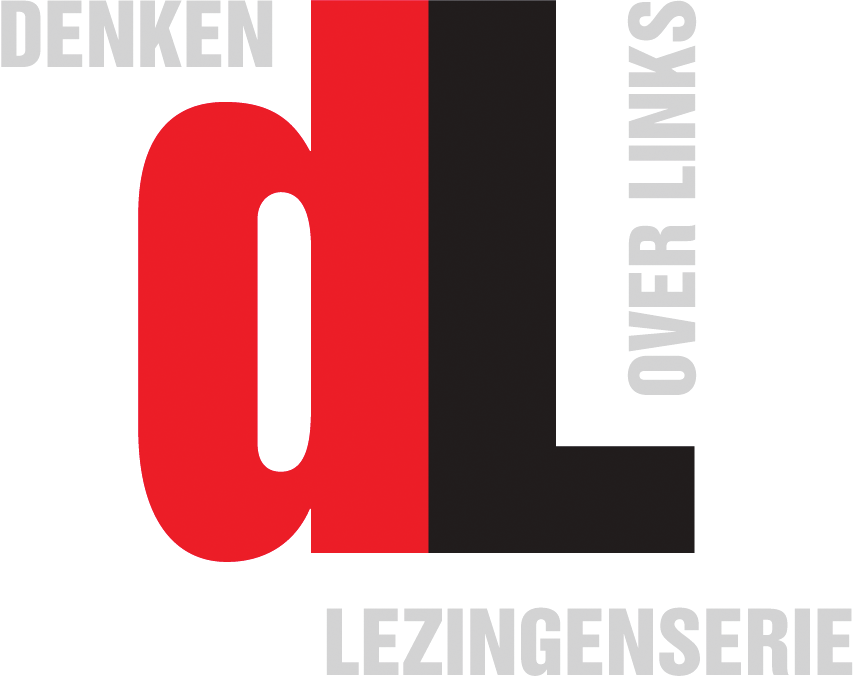
\includegraphics[width=.6\columnwidth]{dol_logo.png}\hfill\begin{tabular}[b]{@{}>{\color{red}\Huge\bf}r@{}}#1\end{tabular}\par
  \myhline \\
  {\bf Gaffelstraat 61B \mysep Toegang gratis \mysep Inloop: 19:30 uur \mysep Start: 20:00 uur \mysep Eind: 22:00 uur} \\
  \myhline
  \par\vspace{7mm}\par
}
 % packages, settings, functions

\begin{document}

\mytitle{.3\columnwidth}{Het gevaar \\ van \\ veiligheid}

\mymega{DONDERDAG 12 SEPTEMBER}

\vfill

\textbf{Onder het motto `denken over links' biedt de SP Rotterdam in haar
nieuwe onderkomen aan de Gaffelstraat een podium voor inspirerende sprekers
over diverse thema's als samenleven in de stad, actief burgerschap, economie en
Europa. Een maandelijkse lezingenserie waarin het denken over hedendaagse
sociale vraagstukken wordt geprikkeld en gescherpt.}

\vfill

\mylarge{Sprekers}

\vfill

\textbf{\large Gwen van Eijk}
\begin{quote}
  Criminoloog en stadssocioloog, verbonden aan de
  Universiteit van Leiden.
\end{quote}

\vfill

\textbf{\large Ren\'e van Swaaningen}
\begin{quote}
  Hoogleraar internationale en comparatieve
  criminologie aan de Erasmus Universiteit Rotterdam,
  directeur van de Erasmus Graduate School of Law en
  voorzitter van de Nederlandse Vereniging voor
  Criminologie (NVK).
\end{quote}

\vfill

\mybox{`Denken over links', een maandelijkse lezingenserie in het SP-pand aan
de Gaffelstraat. Doe mee, denk mee! Iedereen is welkom.}

\newpage

\myhuge{Het gevaar van veiligheid}

\vfill

\textbf{Veiligheid. Het domineert het nieuws, staat op
alle politieke agenda's, en wordt als containerbegrip
voor van alles en nog wat gebruikt en misbruikt.
Iedereen is het erover eens dat we het willen --
immers, wie wil er nou geen veilige samenleving? Maar
wat een veilige samenleving precies is, en hoe deze
moet worden nagestreefd, daarover bestaat minder
eenstemmigheid. Een blik op het gevoerde beleid maakt
snel duidelijk dat onze bewindshebbers veelal de harde
lijn aanhangen, met alle nadruk op repressie.
Cameratoezicht. Preventief fouilleren. Beleid ook dat
steevast de goedkeuring kan wegdragen van "de man in de
straat". Maar werkt het?}

\vfill

Denken over Links begint het nieuwe seizoen met een avond over de keerzijde van
het veiligheidsdenken. De beperking van vrijheden, de stigmatisering en
uitsluiting van groepen. De harde toon waarmee aandacht voor veiligheid gepaard
gaat en het repressieve beleid waarin dit doorsijpelt, hebben het risico het
beoogde doel voorbij te schieten; zozeer zelfs dat ze een negatief effect
hebben op juist de veiligheid en veiligheidsbeleving die ze probeert te
bewerkstelligen. De twee sprekers van deze editie van Denken over Links gaan
dieper in op dit "gevaar van veiligheid". En werpen daarmee gelijk de vraag op
of we de middelen voor het huidige veiligheidsbeleid niet veel effectiever in
kunnen zetten.

\vfill

\textbf{Dr.\ Gwen van Eijk}, criminoloog en stadssocioloog, verbonden aan de
Universiteit van Leiden.
\begin{myquote}
  Er wordt vrijwel geen onderzoek meer gedaan naar `klassenjustitie'; we
  beweren nu dat we in een klasseloze samenleving leven. Maar meer subtiel
  spelen klassenverschillen nog altijd een rol in hoe we denken over bepaalde
  groepen in de samenleving.
\end{myquote}
{\footnotesize NWO Veni-subsidie aanvraag 2013 (toegekend)}

\vfill

\textbf{Prof.\ Dr.\ Ren\'e van Swaaningen}, hoogleraar internationale en comparatieve
criminologie aan de Erasmus Universiteit Rotterdam, directeur van de Erasmus
Graduate School of Law en voorzitter van de Nederlandse Vereniging voor
Criminologie (NVK).
\begin{myquote}
  Terrorisme heeft uiteindelijk te maken met mensen die zich afgewezen en
  vernederd voelen. In een politiestaat zal het moslimradicalisme niet
  verdwijnen.
\end{myquote}
{\footnotesize NRC, 13 November 2004.}

\vfill

Nieuwsgierig? Kom langs en debateer met ons mee op 12 september op de Gaffelstraat.
Aanvang 20:00, deur open 19:30. De toegang is gratis.

\myhline

\end{document}
